\subsubsection{Definition}

A three-dimensional homogeneous aquifer is chosen to verify advective dispersive transport. The side length of the cube model domain is 100 $m$. The velocity field is held constant in the diagonal direction from bottom left to top right (Fig.~\ref{CubeSchematic}).

\begin{figure}[htbp!]
\centering
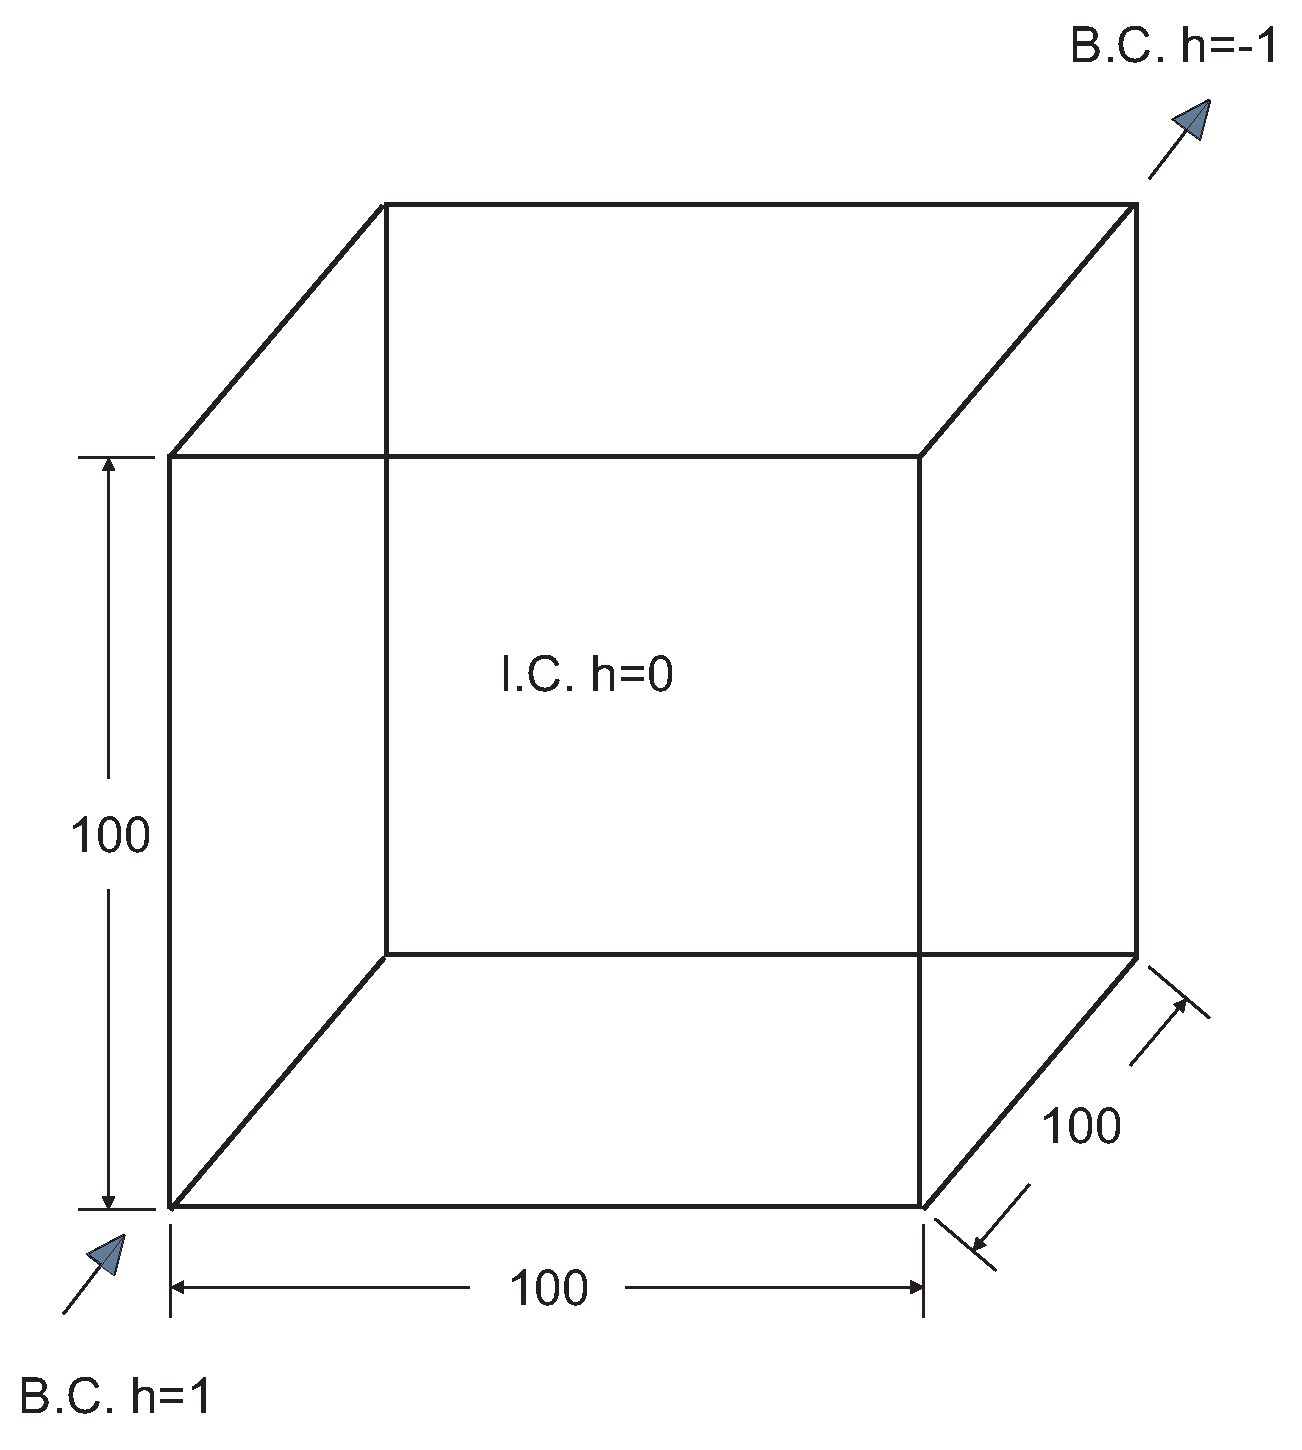
\includegraphics[scale=0.2]{PART_II/C/CubeSchematic.eps}
\caption{Particle tracking in 3D homogeneous aquifer}
\label{CubeSchematic}
\end{figure}

\subsubsection{Analytical solution}

The stated problem can be solved with an analytical solution provided by \cite{aO61}.

\begin{equation}\label{analytical3d}
C\left( {x,y,z,t} \right) = \frac{{C_0 V}}{{8\left(\pi t\right)^{3/2} \sqrt {D_{xx} D_{yy} D_{zz}} }}\exp\left[ { - \frac{{\left( {x - x_0 } \right)^2 }}{{4D_{xx} t}} - \frac{{\left( {y - y_0 } \right)^2 }}{{4D_{yy} t}} - \frac{{\left( {z - z_0 } \right)^2 }}{{4D_{zz} t}}} \right]
\end{equation}

where $C_0$ is the initial concentration.

\subsubsection{Numerical solution}

The domain is discretized with tetrahedral elements. The same grid density is used for converting particle distributions to element concentrations. The head gradient is set by assigning two constant boundary conditions on the diagonal joint points.

The initial source load is applied to an area close to the bottom left of the domain to have an initial concentration of $C _0=1$ $kg m^{-3}$. The material properties for this model setup are given in Tab.~\ref{tab-3dhomo}.

\begin{table}[htbp!]
\caption{\label{tab-3dhomo}Material properties}
\begin{center}
\begin{tabular}{llrr}
\toprule
Symbol & Parameter & Value & Unit \\
\midrule
$k$         & Permeability                    & $6.0804^{-10}$   & m$^{2}$ \\			
$\alpha _L$	& Longitudinal dispersivity       & 0.005              & m \\
$\alpha _T$	& Transverse dispersivity         & 0.005              & m \\
$n$         & Porosity        		            & 0.2                & $-$ \\
\bottomrule
\end{tabular}
\end{center}
\end{table}

\subsubsection{Results}

The advection-dispersion of the particles pulse across the cube is shown in Fig.~\ref{CubeCloud}.

\begin{figure}[htbp!]
\centering
\includegraphics[scale=0.15]{PART_II/C/CubeCloud.eps}
\caption{Particle clouds in the cube}
\label{CubeCloud}
\end{figure}

The result of RWPT simulation for the distribution of concentration over time is compared to the analytical solution. The comparison result is shown in Fig.~\ref{CubeBTC}.

\begin{figure}[htbp!]
\centering
\includegraphics[scale=0.35]{PART_II/C/CubeBTC.eps}
\caption{Breakthrough curves for particle tracking with advection and dispertion}
\label{CubeBTC}
\end{figure}